% Created 2020-05-14 jue 12:30
% Intended LaTeX compiler: pdflatex
\documentclass[presentation,aspectratio=1610]{beamer}
\usepackage[utf8]{inputenc}
\usepackage[T1]{fontenc}
\usepackage{graphicx}
\usepackage{grffile}
\usepackage{longtable}
\usepackage{wrapfig}
\usepackage{rotating}
\usepackage[normalem]{ulem}
\usepackage{amsmath}
\usepackage{textcomp}
\usepackage{amssymb}
\usepackage{capt-of}
\usepackage{hyperref}
\usepackage{khpreamble}
\usepackage{pgfplots}
\usepackage{pdfpages}
\usepackage{circuitikz}
\usepgfplotslibrary{groupplots}
\usetikzlibrary{positioning,circuits.plc.ladder}
\renewcommand*{\not}[1]{\ensuremath{\bar{#1}}}
\renewcommand*{\not}[1]{\ensuremath{\overline{#1}}}
\newcommand*{\coil}[1]{to[short] ++(0.5, 0) node[coordinate] (orig) {} arc [start angle=180, end angle=150,radius=8mm] (orig) arc [start angle=180, end angle=210,radius=8mm] (orig) ++(1cm, 0) node[coordinate] (coilend) {} arc [start angle=0, end angle=30,radius=8mm] (coilend) arc [start angle=0, end angle=-30,radius=8mm] (coilend) to[short] ++(0.5cm, 0) (orig) ++(0.5, 0.8) node {#1}}
\usetheme{default}
\author{Kjartan Halvorsen}
\date{\today}
\title{Logic control of electro-pneumatic systems}
\hypersetup{
 pdfauthor={Kjartan Halvorsen},
 pdftitle={Logic control of electro-pneumatic systems},
 pdfkeywords={},
 pdfsubject={},
 pdfcreator={Emacs 26.3 (Org mode 9.3.6)}, 
 pdflang={English}}
\begin{document}

\maketitle

\section{Intro}
\label{sec:orge60d4be}


\section{Logic control and boolean algebra - simple intro example}
\label{sec:orgbd55af7}
\begin{frame}[label={sec:org7c854ce}]{Cheese pressing example, sequence A+A-}
\begin{center}
\includegraphics[width=0.5\linewidth]{../../figures/cheese-stamping.png}
\end{center}
{\tiny From FESTO Didactic}
\end{frame}

\begin{frame}[label={sec:org330cfec}]{A logic control loop}
\begin{center}
\includegraphics[width=\linewidth]{../../figures/logic-control-loop}
\end{center}
\end{frame}

\begin{frame}[label={sec:org3a16aac}]{Cheese pressing example - Variables}
Activating solenoid UA+ extends the cylinder, activating  UA- retracts the cylinder.
\begin{columns}
\begin{column}{0.5\columnwidth}
\begin{block}{State variable}
\[ x = \begin{cases} 0 & \text{Cylinder retracted}\\1 & \text{Cylinder extended}\end{cases}\]
\end{block}
\begin{block}{Control signal}
\[ u = \begin{bmatrix} u_1\\u_2 \end{bmatrix}, \]
with
\begin{align*}
u_1 &= \begin{cases} 0 & \text{Don't activate UA+}\\1 & \text{Activate UA+ }\end{cases}\\
u_2 &= \begin{cases} 0 & \text{Don't activate UA-}\\1 & \text{Activate UA-}\end{cases}\\
\end{align*}
\end{block}
\end{column}

\begin{column}{0.5\columnwidth}
\includegraphics[width=0.6\linewidth]{../../figures/AplAmin-solenoids.png}
\begin{block}{Command signal}
\[ u_{c} = \begin{cases} 0 & \text{Button unpushed}\\1 & \text{Button pushed}\end{cases}. \]
\end{block}
\end{column}
\end{columns}
\end{frame}
\begin{frame}[label={sec:orgdae007b}]{Cheese pressing example - Plant dynamics and control law}
Activating solenoid UA+ extends the cylinder, activating  UA- retracts the cylinder.
\begin{columns}
\begin{column}{0.5\columnwidth}
\begin{block}{Plant dynamics \(x_{k+1} = g(x_k, u_k)\)}
\begin{center}
\begin{tabular}{|cc|cc|}
\hline
 &  & state & \\
\(u_{1,k}\) & \(u_{2,k}\) & \(x_k\) & \(x_{k+1}\)\\
\hline
0 & 0 & 0 & 0\\
0 & 1 & 0 & 0\\
1 & 0 & 0 & 1\\
1 & 1 & 0 & 0\\
0 & 0 & 1 & 1\\
0 & 1 & 1 & 0\\
1 & 0 & 1 & 1\\
1 & 1 & 1 & 1\\
\hline
\end{tabular}
\end{center}
\end{block}
\end{column}

\begin{column}{0.5\columnwidth}
\begin{block}{Control law \(u_k = f(x, u_c)\)}
\begin{center}
\begin{tabular}{|cc|cc|}
\hline
\(x\) & \(u_{c}\) & \(u_1\) & \(u_2\)\\
\hline
0 & 0 & 0 & 0\\
1 & 0 & 0 & 1\\
0 & 1 & 1 & 0\\
1 & 1 & 0 & 1\\
\hline
\end{tabular}
\end{center}

\begin{align*}
  u_1 &= \qquad\qquad\\
  u_2 &= 
\end{align*}
\end{block}
\end{column}
\end{columns}
\end{frame}
\begin{frame}[label={sec:org168f725}]{Cheese pressing example - implementing the control  law}
\begin{center}
	 \begin{tikzpicture}
	   \node at (-2,0.5) {+24V};
	   \node at (8,0.5) {0V};
	   \draw (-2,0) to[short, o-]  (-2,-3);
	   \draw (8,0) to[short, o-](8,-3);
	   \draw (6, -0.5) \coil{$u_1$};
	   \draw (6,-2.5) \coil{$u_2$};
      \end{tikzpicture}
\end{center}
\begin{center}
  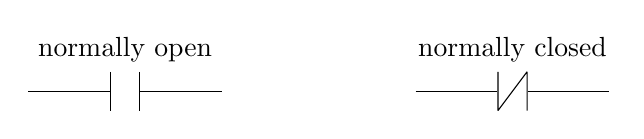
\begin{tikzpicture}[circuit plc ladder,]
    \draw(0,0) to [contact NO={info={normally open}}] ++(2,0);
    \draw(4,0) to [contact NC={info={normally closed}}] ++(2,0);
  \end{tikzpicture}
\end{center}
\begin{center}
  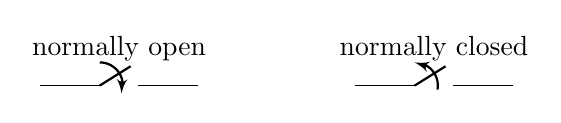
\begin{tikzpicture}
    \draw(0,0) to [switch, label={normally open}] ++(2,0);
    \draw(4,0) to [opening switch, label={normally closed}] ++(2,0);
  \end{tikzpicture}
\end{center}
\end{frame}

\section{Latching circuit}
\label{sec:org0c112cf}
\begin{frame}[label={sec:org6a03413}]{Intermezzo - An electrical circuit with memory}
\begin{columns}
\begin{column}{0.6\columnwidth}
\begin{block}{Latching circuit}
\begin{center}
         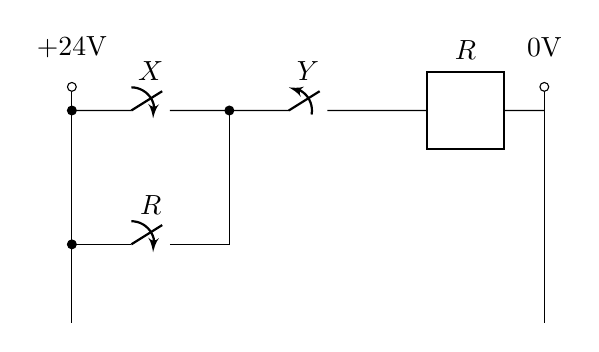
\begin{tikzpicture}
           \node at (0,0.5) {+24V};
           \node at (6,0.5) {0V};
           \draw (0,0) to[short, o-]  (0,-3);
           \draw (6,0) to[short, o-](6,-3);
           \draw (0,-0.3) to[switch, *-, label=$X$] (2,-0.3) to[ opening switch, label=$Y$, ] (4,-0.3) to[short] (4,-0.3) to[twoport, label=$R$] (6,-0.3); %\coil{$R$};
           \draw (0,-2) to[switch, *-, label=$R$] (2,-2)  to[short,-*] (2,-0.3);
         \end{tikzpicture}
\end{center}
\end{block}
\end{column}


\begin{column}{0.4\columnwidth}
\begin{block}{Truth table}
\begin{center}
\begin{tabular}{|ccc|c|}
\(X\) & \(Y\) & \(R_k\) & \(R_{k+1}\)\\
\hline
0 & 0 & 0 & \\
0 & 0 & 1 & \\
0 & 1 & 0 & \\
0 & 1 & 1 & \\
1 & 0 & 0 & \\
1 & 0 & 1 & \\
1 & 1 & 0 & \\
1 & 1 & 1 & \\
\hline
\end{tabular}
\end{center}
\end{block}
\end{column}
\end{columns}
\end{frame}

\section{The lab assignment}
\label{sec:org84149d7}

\begin{frame}[label={sec:org559d99e}]{The lab assignment}
\begin{center}
\includegraphics[width=0.4\linewidth]{../../figures/cheese-pressing-two-cylinders}
 \includegraphics[width=0.58\linewidth]{../../figures/AplusBplusBminAmin}
\end{center}

\begin{center}
\includegraphics[width=0.8\linewidth]{../../figures/logic-control-loop}
\end{center}
\end{frame}


\begin{frame}[label={sec:org9570e2e}]{Implementing the sequence A+B+B-A-}
\begin{center}
\includegraphics[width=0.8\linewidth]{../../figures/AplusBplusBminAmin}
\end{center}
\end{frame}

\begin{frame}[label={sec:orgcc75451}]{Implementing the sequence A+B+B-A-, control signal}
\begin{center}
\includegraphics[width=0.42\linewidth]{../../figures/AplBplBminAmin-pneum.png}
\includegraphics[width=0.58\linewidth]{../../figures/logic-control-loop}
\end{center}

\begin{block}{Control signal}
 \[ u = \begin{bmatrix} u_A+ & u_A- & u_B+ & u_B- \end{bmatrix}^T, \]
 with
 \[ u_A+ = \begin{cases} 0 & \text{Solenoid extending A is not activated}\\
                               1&\text{Solenoid extending A is activated}\\
              \end{cases}
   \]
etc.
\end{block}
\end{frame}

\begin{frame}[label={sec:org84cd8f8}]{Implementing the sequence A+B+B-A-, state variables}
\begin{center}
\includegraphics[width=0.3\linewidth]{../../figures/AplusBplusBminAmin}
\includegraphics[width=0.68\linewidth]{../../figures/logic-control-loop}
\end{center}

\begin{block}{State variables (naive)}
\[ x = \begin{bmatrix} x_A & x_B \end{bmatrix}^T, \]
with
\[ x_{\{A,B\}} = \begin{cases} 0 & \text{Cylinder \{A,B\} retracted}\\
                               1& \text{Cylinder \{A,B\} extended}
                 \end{cases}
   \]
\end{block}
\end{frame}

\begin{frame}[label={sec:org8d7ec46}]{Implementing the sequence A+B+B-A-, control law}
\begin{center}
\includegraphics[width=0.3\linewidth]{../../figures/AplusBplusBminAmin}
\includegraphics[width=0.68\linewidth]{../../figures/logic-control-loop}
\end{center}
\begin{block}{Control law (problematic)}
Ignoring input signal \(u_c\) (no start/stop buttons). Movement should be cyclic

\begin{center}
\begin{tabular}{|cc|cccc|}
\hline
\(x_A\) & \(x_B\) & \(u_A+\) & \(u_A-\) & \(u_B+\) & \(u_B-\)\\
\hline
0 & 0 &  &  &  & \\
1 & 0 &  &  &  & \\
1 & 1 &  &  &  & \\
0 & 1 &  &  &  & \\
\hline
\end{tabular}
\end{center}
\end{block}
\end{frame}



\begin{frame}[label={sec:org85c4849}]{Implementing the sequence A+B+B-A-, control law}
\begin{center}
\includegraphics[width=0.3\linewidth]{../../figures/AplusBplusBminAmin}
\includegraphics[width=0.68\linewidth]{../../figures/logic-control-loop}
\end{center}
\begin{block}{Control law (problematic)}
Ignoring input signal \(u_c\). Movement should be cyclic

\begin{center}
\begin{tabular}{|cc|cccc|}
\hline
\(x_A\) & \(x_B\) & \(u_A+\) & \(u_A-\) & \(u_B+\) & \(u_B-\)\\
\hline
0 & 0 & 1 & 0 & 0 & 0\\
1 & 0 & 0 & 1 or 0 & 0 or 1 & 0\\
1 & 1 & 0 & 0 & 0 & 1\\
(0) & (1) & 0 & 0 & 0 & 1\\
\hline
\end{tabular}
\end{center}
\end{block}
\end{frame}



\begin{frame}[label={sec:orgb489c40}]{Implementing the sequence A+B+B-A-, the problem}
\alert{The correct control signal (action) is not uniquely defined by the position of the cylinders}
\begin{center}
\includegraphics[width=0.5\linewidth]{../../figures/AplusBplusBminAmin}\\
\includegraphics[width=0.8\linewidth]{../../figures/logic-control-loop}
\end{center}
\end{frame}

\begin{frame}[label={sec:orgbd7ced9}]{Implementing the sequence A+B+|B-A-}
\alert{Dividing the sequence into groups (a.k.a. cascade method)}
\[ \underbrace{\text{A+B+}}_{\text{Group 1}}| \underbrace{\text{B-A-}}_{\text{Group 2}} \]
 \begin{center}
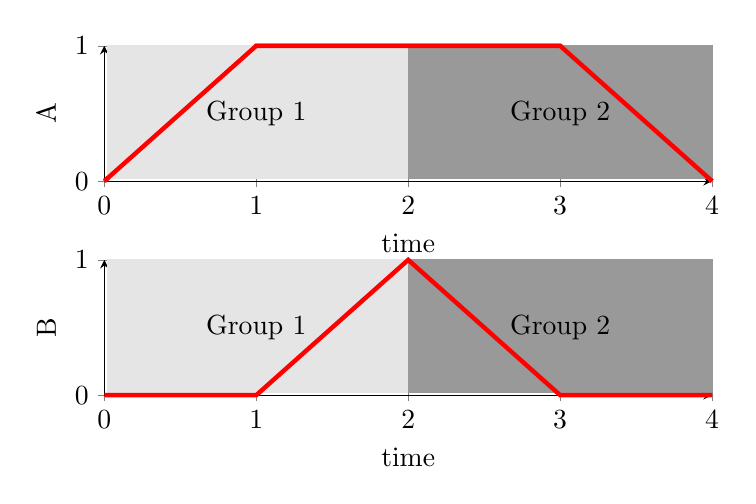
\begin{tikzpicture}
%\pgfplotsset{set layers=default}
  \begin{groupplot} [
    group style={
      group name=timeplot,
      group size=1 by 2,
      xlabels at=all,
      horizontal sep=1cm,
      vertical sep=1cm,
    }, 
    clip=false,
    height=3.3cm, width=9.3cm,
    axis line style={->},
    axis lines=left,
    xlabel={time },
    ylabel={},
    ytick={0,1},
    xtick={0,1,2,3,4},
    % grid=both,
    % xtick=\empty,
    % ytick=\XNOLL,
    % yticklabel=$x_0$,
    ]
    \nextgroupplot [ylabel={A},]
    \addplot[red, no marks,ultra thick,] coordinates {(0,0) (1,1) (2, 1) (3,1) (4, 0)};
    \draw[color=black!10, fill=black!10] (axis cs: 0.02,0.02) rectangle (axis cs: 2,1);
    \node at (axis cs: 1, 0.5) {Group 1};
    \draw[color=black!40, fill=black!40] (axis cs: 2,0.02) rectangle (axis cs: 4,1);
    \node at (axis cs: 3, 0.5) {Group 2};
    \addplot[red, no marks,ultra thick,] coordinates {(0,0) (1,1) (2, 1) (3,1) (4, 0)};

    \nextgroupplot [ylabel={B},]
    \draw[color=black!10, fill=black!10] (axis cs: 0.02,0.02) rectangle (axis cs: 2,1);
    \node at (axis cs: 1, 0.5) {Group 1};
    \draw[color=black!40, fill=black!40] (axis cs: 2,0.02) rectangle (axis cs: 4,1);
    \node at (axis cs: 3, 0.5) {Group 2};
    \addplot[red, no marks,ultra thick,] coordinates {(0,0) (1,0) (2, 1) (3,0) (4, 0)};
  \end{groupplot}
\end{tikzpicture}
  \end{center}
\end{frame}


\begin{frame}[label={sec:orgd4ee8e6}]{Implementing the sequence A+B+|B-A-, state variables}
\begin{columns}
\begin{column}{0.45\columnwidth}
\begin{block}{State variables (better)}
\[ x = \begin{bmatrix} x_A & x_B & x_{G1} & x_{G2}\end{bmatrix}^T, \]
with
 \begin{align*}
  x_{\{A,B\}} &= \begin{cases} 0 & \text{Cylinder \{A,B\} retracted}\\
                            1& \text{Cylinder \{A,B\} extended}
              \end{cases}\\
 x_{Gi} &= \begin{cases} 0 & \text{Group \(i\) not active}\\
                            1& \text{Group \(i\) active}
              \end{cases}
\end{align*}
\end{block}
\end{column}

\begin{column}{0.55\columnwidth}
\begin{block}{State transitions}
 \begin{center}
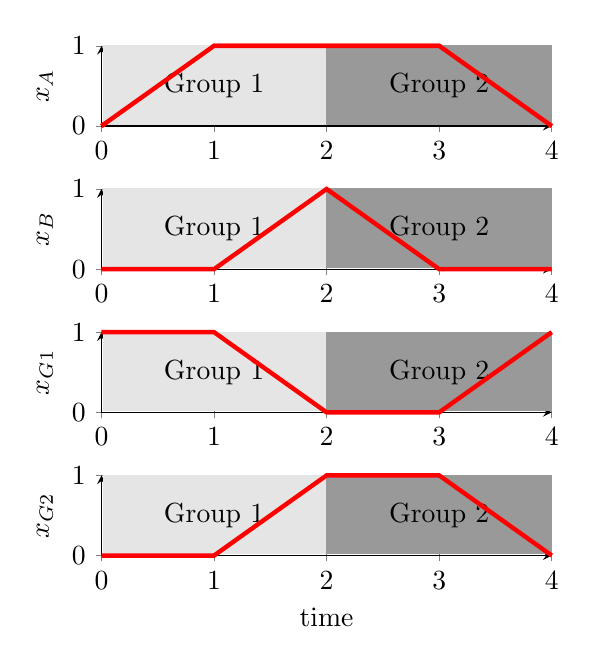
\begin{tikzpicture}
%\pgfplotsset{set layers=default}
  \begin{groupplot} [
    group style={
      group name=timeplot,
      group size=1 by 4,
      xlabels at=edge bottom,
      horizontal sep=1cm,
      vertical sep=8mm,
    }, 
    clip=false,
    height=2.6cm, width=7.3cm,
    axis line style={->},
    axis lines=left,
    xlabel={time },
    ylabel={},
    ytick={0,1},
    xtick={0,1,2,3,4},
    % grid=both,
    % xtick=\empty,
    % ytick=\XNOLL,
    % yticklabel=$x_0$,
    ]
    \nextgroupplot [ylabel={$x_A$},]
    \addplot[red, no marks,ultra thick,] coordinates {(0,0) (1,1) (2, 1) (3,1) (4, 0)};
    \draw[color=black!10, fill=black!10] (axis cs: 0.02,0.02) rectangle (axis cs: 2,1);
    \node at (axis cs: 1, 0.5) {Group 1};
    \draw[color=black!40, fill=black!40] (axis cs: 2,0.02) rectangle (axis cs: 4,1);
    \node at (axis cs: 3, 0.5) {Group 2};
    \addplot[red, no marks,ultra thick,] coordinates {(0,0) (1,1) (2, 1) (3,1) (4, 0)};

    \nextgroupplot [ylabel={$x_B$},]
    \draw[color=black!10, fill=black!10] (axis cs: 0.02,0.02) rectangle (axis cs: 2,1);
    \node at (axis cs: 1, 0.5) {Group 1};
    \draw[color=black!40, fill=black!40] (axis cs: 2,0.02) rectangle (axis cs: 4,1);
    \node at (axis cs: 3, 0.5) {Group 2};
    \addplot[red, no marks,ultra thick,] coordinates {(0,0) (1,0) (2, 1) (3,0) (4, 0)};

    \nextgroupplot [ylabel={$x_{G1}$},]
    \draw[color=black!10, fill=black!10] (axis cs: 0.02,0.02) rectangle (axis cs: 2,1);
    \node at (axis cs: 1, 0.5) {Group 1};
    \draw[color=black!40, fill=black!40] (axis cs: 2,0.02) rectangle (axis cs: 4,1);
    \node at (axis cs: 3, 0.5) {Group 2};
    \addplot[red, no marks,ultra thick,] coordinates {(0,1) (1, 1) (2,0) (3, 0) (4,1)};

    \nextgroupplot [ylabel={$x_{G2}$},]
    \draw[color=black!10, fill=black!10] (axis cs: 0.02,0.02) rectangle (axis cs: 2,1);
    \node at (axis cs: 1, 0.5) {Group 1};
    \draw[color=black!40, fill=black!40] (axis cs: 2,0.02) rectangle (axis cs: 4,1);
    \node at (axis cs: 3, 0.5) {Group 2};
    \addplot[red, no marks,ultra thick,] coordinates {(0,0) (1, 0) (2,1) (3, 1) (4,0)};
  \end{groupplot}
\end{tikzpicture}
  \end{center}
\end{block}
\end{column}
\end{columns}
\end{frame}

\begin{frame}[label={sec:org7e6d85e}]{Implementing the sequence A+B+|B-A-, control law}
\begin{columns}
\begin{column}{0.38\columnwidth}
\begin{block}{State transitions}
 \begin{center}
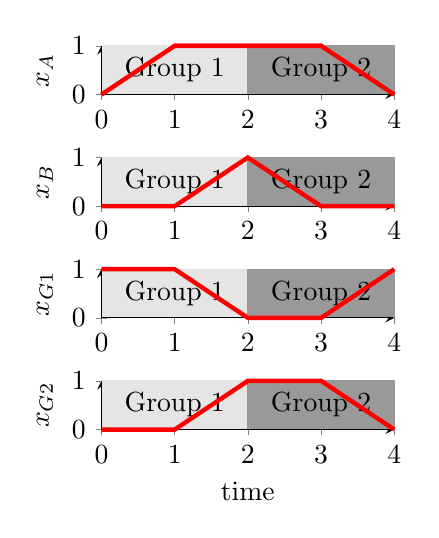
\begin{tikzpicture}
%\pgfplotsset{set layers=default}
  \begin{groupplot} [
    group style={
      group name=timeplot,
      group size=1 by 4,
      xlabels at=edge bottom,
      horizontal sep=1cm,
      vertical sep=8mm,
    }, 
    clip=false,
    height=2.2cm, width=5.3cm,
    axis line style={->},
    axis lines=left,
    xlabel={time },
    ylabel={},
    ytick={0,1},
    xtick={0,1,2,3,4},
    % grid=both,
    % xtick=\empty,
    % ytick=\XNOLL,
    % yticklabel=$x_0$,
    ]
    \nextgroupplot [ylabel={$x_A$},]
    \addplot[red, no marks,ultra thick,] coordinates {(0,0) (1,1) (2, 1) (3,1) (4, 0)};
    \draw[color=black!10, fill=black!10] (axis cs: 0.02,0.02) rectangle (axis cs: 2,1);
    \node at (axis cs: 1, 0.5) {Group 1};
    \draw[color=black!40, fill=black!40] (axis cs: 2,0.02) rectangle (axis cs: 4,1);
    \node at (axis cs: 3, 0.5) {Group 2};
    \addplot[red, no marks,ultra thick,] coordinates {(0,0) (1,1) (2, 1) (3,1) (4, 0)};

    \nextgroupplot [ylabel={$x_B$},]
    \draw[color=black!10, fill=black!10] (axis cs: 0.02,0.02) rectangle (axis cs: 2,1);
    \node at (axis cs: 1, 0.5) {Group 1};
    \draw[color=black!40, fill=black!40] (axis cs: 2,0.02) rectangle (axis cs: 4,1);
    \node at (axis cs: 3, 0.5) {Group 2};
    \addplot[red, no marks,ultra thick,] coordinates {(0,0) (1,0) (2, 1) (3,0) (4, 0)};

    \nextgroupplot [ylabel={$x_{G1}$},]
    \draw[color=black!10, fill=black!10] (axis cs: 0.02,0.02) rectangle (axis cs: 2,1);
    \node at (axis cs: 1, 0.5) {Group 1};
    \draw[color=black!40, fill=black!40] (axis cs: 2,0.02) rectangle (axis cs: 4,1);
    \node at (axis cs: 3, 0.5) {Group 2};
    \addplot[red, no marks,ultra thick,] coordinates {(0,1) (1, 1) (2,0) (3, 0) (4,1)};

    \nextgroupplot [ylabel={$x_{G2}$},]
    \draw[color=black!10, fill=black!10] (axis cs: 0.02,0.02) rectangle (axis cs: 2,1);
    \node at (axis cs: 1, 0.5) {Group 1};
    \draw[color=black!40, fill=black!40] (axis cs: 2,0.02) rectangle (axis cs: 4,1);
    \node at (axis cs: 3, 0.5) {Group 2};
    \addplot[red, no marks,ultra thick,] coordinates {(0,0) (1, 0) (2,1) (3, 1) (4,0)};
  \end{groupplot}
\end{tikzpicture}
  \end{center}
\end{block}
\end{column}


\begin{column}{0.62\columnwidth}
\begin{block}{Control law}
\begin{center}
\begin{tabular}{|cccc|cccc|}
\hline
\(x_A\) & \(x_B\) & \(x_{G1}\) & \(x_{G2}\) & \(u_A+\) & \(u_A-\) & \(u_B+\) & \(u_B-\)\\
\hline
0 & 0 & 1 & 0 &  &  &  & \\
1 & 0 & 1 & 0 &  &  &  & \\
1 & 1 & 0 & 1 &  &  &  & \\
1 & 0 & 0 & 1 &  &  &  & \\
\hline
\end{tabular}
\end{center}
\end{block}
\end{column}
\end{columns}
\end{frame}


\begin{frame}[label={sec:org14f0fa7}]{Implementing the control law}
\begin{center}
         \begin{tikzpicture}
           \node at (-2,0.5) {+24V};
           \node at (8,0.5) {0V};
           \draw (-2,0) to[short, o-]  (-2,-7);
           \draw (8,0) to[short, o-](8,-7);
	   \draw (6, -0.5) to[twoport, label={$u_{A+}$}] (8,-0.5); %\coil{$u_{A+}$};
           \draw (6,-2.5) to[twoport, label={$u_{A-}$}] (8,-2.5);%\coil{$u_{A-}$};
	   \draw (6, -4.5) to[twoport, label={$u_{B+}$}] (8,-4.5);%\coil{$u_{B+}$};
           \draw (6,-6.5) to[twoport, label={$u_{B-}$}] (8,-6.5);% \coil{$u_{B-}$};
      \end{tikzpicture}
\end{center}
\end{frame}


\begin{frame}[label={sec:org0aa38da}]{Implementing the group transitions}
\begin{center}
         \begin{tikzpicture}
           \node at (-2,0.5) {+24V};
           \node at (8,0.5) {0V};
           \draw (-2,0) to[short, o-]  (-2,-7);
           \draw (8,0) to[short, o-](8,-7);
	   \draw (6, -0.5) to[twoport, label={$x_{G1}$}] (8,-0.5);%\coil{$x_{G1}$};
	   \draw (6, -4.5) to[twoport, label={$x_{G2}$}] (8,-4.5);%\coil{$x_{G2}$};
	   \draw (-2,-2) to[switch, *-, label={$x_{G1}$}] (1,-2);
	   \draw (-2,-6) to[switch, *-, label={$x_{G2}$}] (1,-6);
      \end{tikzpicture}
\end{center}
\end{frame}



\begin{frame}[label={sec:org163444c}]{Implementing the proximity sensor circuit}
\begin{center}
\includegraphics[height=0.9\textheight]{sensor-circuit}
\end{center}
\end{frame}
\end{document}